%
% additional usepackage{beamerthemeshadow} is used
\documentclass{beamer}
\usepackage[utf8]{inputenc}
\usepackage{graphics}
\usepackage{ccicons}
\usepackage[ngerman]{babel}
\usepackage{pdfpages}
%\usepackage{beamerthemeshadow}
\usetheme{Montpellier}
\begin{document}

	\title{ 
Ein 2. Leben für meinen betagten PC/Laptop }  
	\author{HG Unckell\hspace{5mm}
	\raisebox{-10mm}{
\includegraphics[height=3cm]{LogoCTB}}
 }
	\date{11. Januar 2023 - \ccby} 
	
	\frame{\titlepage} 
		\logo{
\includegraphics[height=1.2cm]{LogoCTB}}
	\frame{\frametitle{Übersicht}\scriptsize\tableofcontents} 
	
	\section{Ausgangspunkt - Was ist das Interesse?} 
	\subsection{Nutzung eines funktionsfähigen Geräts}
	\frame{ \frametitle{Vorgabe von Microsoft}
		
\includegraphics[width=\columnwidth]{Windows11Logo}
		
		Die aktuelle Version des Microsoft-Betriebssystems (seit Oktober 2021) hat einige Hardware-Anforderungen,
die dazu führen können,
dass man nicht gut auf dieses Betriebssystem umsteigen kann.
}

\frame{ \frametitle{Warum gibt es überhaupt solche Generationen?}

Wer ein  Betriebssystem kauft / installiert,
braucht für die Nutzungsdauer die Pflege des Systems.\bigskip

Microsoft bietet ca. 10 Jahre dafür   an.
\begin{itemize}
	\item 

Windows 7 -- Oktober 2009 Einführung

Januar 2020 Ende des  Support
\item 
Windows 8.1 -- November 2013 Einführung 

Januar 2023 Ende des  Support
\item 
Windows 10 -- Juli 2015 Einführung

Oktober 2025  Ende des  Support
\end{itemize}
}

\frame{ \frametitle{Was bedeutet ein Umstieg auf die nächste Generation?}


Wenn der Support endet, wird ein Umstieg nötig,
wenn das Gerät mit der Außenwelt, z.B. über das Internet
Kontakt hat. 
\bigskip

Die nächste Generation eines Betriebssystem stellt meist höhere Anforderungen an die Hardwarefähigkeiten
eines Geräts. D.h. oft muss ein neues Gerät gekauft werden.\bigskip

Eine Entwicklung, die bei den Smartphones noch extremer verläuft, und die
aus der Sicht der Nachhaltigkeit, des ökologischen Fußabdrucks, problematisch ist.
Das Projekt ,,Upcycling Android'' adressiert dieses Anliegen, mehr dazu unter
https://upcycling-android.org
}
\section{Blick auf die Hardwareentwicklung}

\frame{ \frametitle{Immer schneller --
Warum veraltet so ein Gerät so schnell?}

Um die Hintergründe besser zu verstehen, einzuordnen,

nun ein kurzer Blick in die Geschichte.
\bigskip

Es gibt als Faustregel das \textbf{\textsf{mooresche Gesetz}}:

Alle \textbf{\textsf{x}} Jahre verdoppelt sich die Komplexität der in den PCs genutzten Schaltkreise,
d.h. die Fähigkeit der Geräte. 

(je nach Quelle ist x 1, 1.5 oder 2)
\bigskip

D.h. neue Geräte können schnell viel mehr und das machen die Betriebssystemgenerationen
nutzbar.

Und natürlich rufen manche Nutzer diese Leistung auch ab, z.B. beim Spielen. So gibt es einen Anstoß, ein neues Gerät zu kaufen.
}
\subsection{Gang durch die Geschichte in 10 Jahresschritten}
\frame{ \frametitle{Eigene Erfahrung damit -- zur Illustration }

1975 habe ich meine Lehre als Programmierer begonnen.
Damals wurde der Abteilungsrechner von der IBM gerade auf 1024 KB Kernspeicher aufgerüstet.
\bigskip

Die Nutzung des Prozessrechner PDP8 war  von Effizienzfragen getrieben.
5 - 10 Nutzer  konnten
 an diesem System arbeiteten.
 
\bigskip Zur Arbeit mit einem Computers habe ich mir oft
etwas angezogen, da die Räume klimatisiert, also im Sommer ziemlich kalt waren.
 
\bigskip
Die Möglichkeiten, die sich durch die Entwicklung bei der Hardware ergaben,
sind wirklich bedeutsam. Unterschiedlich große Buchstaben,
etwas, was heute ganz normal für ein Textdokument ist, waren unvorstellbar.
}

\frame{ \frametitle{Graphische Oberflächen werden möglich}

10 Jahre später wurde mit dem  Apple Macintosh ein
persönlicher Computer mit graphischer Oberfläche
 für Privatleute erschwinglich. 
 
 Diese Möglichkeiten machen einen großen
Unterschied für die Bedienbarkeit aus. Erschwinglich meint rund 10 000 DM. \bigskip

10 Jahre später ist bei Windows 95  die graphische Benutzeroberfläche  Standard.\bigskip

10 Jahre später kommt  Windows Vista auf den Markt.

Ein deutlich komplexeres Betriebssystem --
Wikipedia  dazu:

Nach einer Schätzung des amerikanischen Wirtschaftsmagazins BusinessWeek hatte Microsoft 5 Jahre lang rund 10.000 Angestellte für das Projekt eingesetzt und etwa 10 Milliarden US-Dollar in die Entwicklung investiert.
}
\subsection{Grenzen des Wachstums}
\frame{ \frametitle{Sinkender Zusatznutzen von zusätzlicher Leistung}

Spätestens zu dieser Zeit erleben viele einfache Nutzer

 \begin{center}
 	\textbf{\textsf{das Gesetz des abnehmenden Ertrags.}}
 \end{center}
 
Das bisherige  Gerät reicht gut aus für 
 Tätigkeiten, wie Dokumente erstellen, Medien abspielen, im Internet surfen, Email, $\ldots$.
\bigskip

Videos schneiden oder andere rechenintensiven Aufgaben
sind nicht im Blick, brauchen daher auch keine 
Unterstützung - könnten gleichzeitig, durch die Entwicklung bei  Smartphones etc.  zu einem 
neuen Bedarf führen.
}
\section{Der persönliche Computer}
\subsection{Kulturfragen - Potential einer kreativen Kultur des Gebens}
\frame{ \frametitle{Der persönliche Computer - PC - als Möglichkeit}

Jetzt soll etwas in den Blick kommen, was das Werden der  PCs, der persönlichen Computern mit bewirkt hat.
Ein PC ermöglicht Dinge zu tun, die sonst nur große Firmen machen können.  1979 machte Apple II z.B.  Tabellenkalkulation (Visicalc) verfügbar.
\bigskip

Einflussreichen Personen der ersten 
Entwicklergeneration war die damit zugängliche Freiheit ein zentrales Anliegen.
So bildet sich das Konzept des \textbf{\textsf{Copyleft}}, anstatt von Copy\textbf{\textit{right}} heraus.

Die Macher dieser Software-güter wollen diese der Gesellschaft geben, so   soziale Solidarität fördern ‑ also gemeinsame Nutzung und Zusammenarbeit.
 Copyleft entsteht (sehr vereinfacht) als Richtlinie, die verhindert, dass beim weiteren Verteilen des Programms keine Restriktionen hinzugefügt werden können, um Anderen wesentliche Freiheiten zu versagen. 
%Diese Richtlinie widerspricht nicht den wesentlichen Freiheiten ‑ vielmehr schützt es sie. 
}
\frame{ \frametitle{Freiheit - Floskel des Jahres 2022}
	Der FSF, der free - software - foundation,
	ist bewusst, der Begriff Freiheit kann unterschiedlich gefüllt werden. Mehr dazu u.a. auf \url{https://fsfe.org}.  Richard Stallmann, der Gründer dieser Stiftung, hat 
vier wesentliche Freiheiten
freie Software beschrieben:

Die Freiheit (0 - Verwenden), das Programm auszuführen wie man möchte, für jeden Zweck.

Die Freiheit (1 - Verstehen), die Programmfunktion  zu untersuchen und eigenen Datenverarbeitungbedürfnissen anzupassen. 
%Der Zugang zum Quellcode ist dafür Voraussetzung.

Die Freiheit (2 - Verbreiten), das Programm weiter zu geben und damit Mitmenschen zu helfen.

Die Freiheit (3 - Verbessern), das Programm zu verbessern und diese Verbesserungen der Öffentlichkeit freizugeben, damit die gesamte Gesellschaft davon profitiert. 
%Der Zugang zum Quellcode ist dafür Voraussetzung.
	
	
%Die ersten PCs, wie der Apple II, entstanden in einer alternativen  auch etwas anarchischen Kultur.
%Da ist z.B von \textbf{\textsf{Copyleft}}, anstatt von Copyright die Rede.
%Wichtige auch soziale Impulse dieser Kultur zeigen sich als FSF gegründet von Richard Stallmann - einer schillernden Person, wenn man 
%dazu in der Wikipedia nachliest.
%\bigskip


}

\frame{ \frametitle{Digitale Wertschöpfung ist anders}
	
	 Digitalen Güter unterscheiden sich grundlegend von analogen.
	 Programme können durch  Nutzung besser werden. Fehler werden
	 sichtbar \& könnten behoben werden, Kopien  sind nahezu umsonst.
	\bigskip
	
Erst  
 freie Anwendungen entstanden in der Textverarbeitung. Diese Programme laufen auf unterschiedlichen
Betriebssystemen und vermeiden einen Lock-in Effekt. D.h. 
eigene Daten sind
 auf einem anderen System  weiter nutzbar. Seit über 30 Jahren nutze ich  das Textsatzsystem \TeX z.B. auch für diese Folien. Frei heißt nicht kostenlos - es braucht  für alle, die daran arbeiten und so etwas der Menschheit geben, Finanzierungsmodelle, z.B. Nutzergruppen. \bigskip

%D.h. seit 35 Jahren gibt es ein Archiv von
%Texten, dass ich auf vielen Systemen nutzen kann.
Sie haben vielleicht schon mal \textbf{\textsf{LibreOffice}} oder \textbf{\textsf{Firefox}} genutzt.	
	

}

\frame{ \frametitle{Downsizing beginnt}
		
	Ab Mitte der 90iger Jahre ermöglicht die allgemein verfügbare
	Internetnutzung eine Vergemeinschaftung von Programmierern
	in einer  neuen Qualität. 
	Eine produktive Hacker-Kultur entsteht.\bigskip
	

Das mooresche Gesetz hat auch die andere Richtung:
Rechenleistung wird immer preiswerter.

\bigskip
In den 90iger Jahren entsteht das Betriebssystem LINUX und macht Funktionen  professioneller, teurer Workstations, 
auf den PCs mit inzwischen ausreichender Rechenleistung dafür, verfügbar. Vorarbeiten dazu ab 1984 im GNU-projekt \url{https://gnu.org}.

\bigskip Die Alternative GNU/Linux half
dann Nutzern von Windows 95, ihre Geräte 
länger im Einsatz zu haben.
}

\frame{ \frametitle{FLOSS - freie offene Software}
	
	Die Rechtssituation für diese Alternativen ist durch die 4 Freiheiten so,
	dass man sie nicht kaufen kann. Man darf sie nutzen, kann für Dienstleistungen mit 
	dieser Software Geld verlangen. 
	
\bigskip
Oft entstehen solche Programme im Umfeld von
Universitäten.

\bigskip
Public money - public code
ist eine wichtige Bewegung für das Bereitstellen
und auch das Nutzen dieser Programme.

\bigskip
Wichtige Bereiche des Internets sind ohne
FLOSS nicht zu denken.	
}

\frame{ \frametitle{Linux ist attraktive Basis}
	
	Heute ist das meistgenutzte Betriebssystem Android, das übrigens auch diese Konzepte
	aufnimmt, also einen Linux-Kern hat und damit freie Software nutzt.
	
	
\includegraphics[width=60mm]{android-logo}
	
	Oft werden auch nicht freie Programme auf dem
	Smartphone installiert - und es entsteht ein 
	Lock-in Effekt mit Google.
}

\section{Nutzung ohne Lock-in Effekt}

\frame{ \frametitle{Bewährte Alternative}
Es gibt viele Gründe, sein Gerät mit 
Programmen zu nutzen, die offenen Standards folgen,
keine Daten der Nutzer abgreifen und
eine maximale Lebensdauer der Hardware
ermöglichen.\bigskip

Eine Alternative zur Betriebssystemfamilie 

von Microsoft - LINUX - wird von einem 

Kollektiv unterschiedlicher Personen erstellt.

\vspace{-18mm}

\hfill
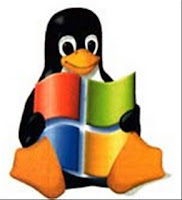
\includegraphics[width=23mm]{linux-windows.jpg}
%\bigskip

Diverse Firmen sowie große Verwaltungen haben  ein Interesse,
sich nicht zu sehr an einen Hersteller zu binden, selber Anpassungen vornehmen zu können.
Das geht bei Programmen mit offenem Quellcode   naturgemäß viel einfacher.
Gerade die Freiheiten 2+3 ergeben für diese Firmen eine spürbare Kostenentlastung.
}

\frame{ \frametitle{Standardausstattung}

Neben dem Betriebssystem, welches geschichtlich gesehen, als letzte Ebene dazukam,
gibt es die Ebene der wichtigen Anwendungen, bei der gute, frei verfügbare Alternativen existieren.
%\bigskip
\begin{itemize}
	\item 
\textbf{\textsf{LibreOffice}} für die wichtigsten Aufgaben im Büro
\item 
\textbf{\textsf{Firefox}} als Browser, also dem Umgang im Internet
\item 
\textbf{\textsf{Thunderbird}} für die Email-Nutzung
\item 
\textbf{\textsf{GIMP}} für die Bildbearbeitung.
\item \textbf{\textsf{Wine}} um ältere Windowsprogramme zu nutzen.
\end{itemize}
Die üblichen Drucker / Scanner werden oft automatisch erkannt.
D.h. eine Standardnutzung  ist mit betagten Geräten gut zu machen.
}
\subsection{Migration leicht gemacht}
\frame{ \frametitle{Verfügbare Unterstützung}

Wer  auf seinem Gerät Linux installiert,
profitiert von einer großen Community, d.h.  Foren mit Tipps und der Möglichkeit,
 das eigene Problem in einer der vielen Fragen und Antworten wieder zu finden.

%\bigskip
Es gibt ein Anzahl von Systemzusammenstellungen, Distributionen.
Typische Unterschiede liegen z.B
\begin{itemize}
	\item 
in der Art und Weise,
wie  neue Impulse aufgegriffen werden.

Wo ist Priorität? 
Stabilität $\Longleftrightarrow$
 neue Funktionen
\item 
in den Möglichkeiten, das System zu
verändern. Bedienungsfreundlichkeit für Anfänger
 $\Longleftrightarrow$
 Flexibilität  
\end{itemize} 
%
%Je nach Vorliebe passt die eine oder die andere Art mehr.

%\bigskip
Dazu finden sich im Netz oder auch in  entsprechenden Zeitschriften  Hinweise. Zeitschriften haben 
oft auch einen Datenträger, der es  ermöglicht, das neue System einmal auszuprobieren.

}
\frame{ \frametitle{Konkrete Schritte - Planung}
	Wer eine Migration, also den Umstieg auf
	LINUX anstrebt, sollte sich  bewusst sein,
	\textbf{\textsf{Selbstwirksamkeit}} ist in dieser Kultur  sehr wichtig.
	D.h. es gibt gerne Hilfe zum Starten.
	
	Es wird ebenso erwartet, dass man sich in Foren und anderen Medien schlau macht. \bigskip
	
	Folgende Entscheidungen/Klärungen stehen dazu an:
%	 sind dann zu treffen:
	\begin{itemize}
\item Welche Anwendungen sollen genutzt werden?
	\item Welche Hardwareressourcen stellt das
	Gerät zur Verfügung?
		\item 
Welche Distribution passt dazu?
	\end{itemize}	

}
\frame{ \frametitle{Konkrete Schritte - Vorarbeit}

Wie bei einem Umzug im echten Leben,
ist eine solche Migration der Anlass,
das Bestehende, in diesem Fall die vorhandenen
Daten zu sichten und Wichtiges so zu sichern,
dass es auf dem neuen System wieder
verfügbar gemacht werden kann.

\bigskip
Bilder und weitere Medien nicht vergessen!

\bigskip
Heute bietet sich dafür ein USB-Stick an.

\bigskip
\textbf{\textsf{\Large Achtung:}} die Passwörter, die im Browser und anderen Anwendungen gespeichert sind, gehen bei der Migration natürlich auch verloren.

\bigskip
Beratung/Begleitung im CTB natürlich möglich.

}
\frame{ \frametitle{Konkrete Schritte - Neuinstallation}
	
	Für die gewählte Distribution muss
	ein Installationsmedium vorliegen.
	\begin{itemize}
		\item 
	 ein USB-Stick mit der  aktuellsten 
	Version aus dem Netz 
	\item 
	 eine DVD aus einer Zeitschrift 
\end{itemize}
Von diesem Medium wird das Gerät gebooted,
also gestartet.

Dazu muss evtl. die Reihenfolge der Bootmedien
verändert werden.

Es fährt die Distribution vom Bootmedium hoch.
Man kann ausprobieren, ob ein erster Test klappt
und dann Linux installieren.

Wenn genug Platz auf der Festplatte ist, 
kann sogar meist das alte System bleiben, 
und es ist möglich, auf die bisherigen Daten
größtenteils noch zuzugreifen (aber nicht ganz unkompliziert).

Sinnvoll ist auf jeden Fall, 
die gesicherten Daten einzuspielen...
}

\end{document}


